\documentclass[runningheads]{llncs}

\usepackage[T1]{fontenc}
\usepackage{lmodern}
\usepackage{graphicx}
\usepackage{amsmath,amssymb}
\usepackage{booktabs}
\usepackage{multirow}
\usepackage{xcolor}
\usepackage{pifont}
\usepackage{url}
\usepackage{hyperref}
\usepackage{cite}
\usepackage{microtype}
\usepackage{indentfirst}

\hypersetup{colorlinks=true,linkcolor=blue,urlcolor=blue,citecolor=blue,pdfauthor={},pdftitle={PRISM: Confidential Smart Contract Auditing with Pseudonymized Graph Screening}}
\setlength{\tabcolsep}{5pt}
\newcommand{\cmark}{\ding{51}}
\newcommand{\xmark}{\ding{55}}

\begin{document}

\title{PRISM: Confidential Smart Contract Auditing with Pseudonymized Graph Screening}
\titlerunning{PRISM: Confidential Smart Contract Auditing}

\author{Anonymous Author(s)}
\authorrunning{Anonymous}
\institute{Anonymous Institution}

\maketitle

\begin{abstract}
Hosted language models make smart-contract audits disclose unreleased source code and business logic. We present PRISM, a confidential audit pipeline whose trust boundary is the audit host. PRISM strips secrets and reversibly pseudonymizes identifiers, turns Slither's static single assignment (SSA) intermediate representation into typed function-level code property graphs (CPGs), screens and ranks functions with a two-stage graph attention model, audits the highest-ranked functions with a locally served open-weight code LLM, and validates reference harnesses with Foundry on a local EVM, restoring identifiers only in the final report. On 12,991 public function graphs covering five Smart Contract Weakness Classification (SWC) classes, the ranker reaches $75.95\pm0.19\%$ macro-F1 on a random split and $76.31\pm0.06\%$ on a lineage-disjoint split over five seeds, at 0.21\,ms per function. Graph convolutional and graph isomorphism baselines reach the same level, share at least 97\% of its errors and differ in none of 20 paired tests, indicating that contract-derived labels likely dominate the remaining error. On 57 contracts, pseudonymization preserves compilation and every Slither detector type, but a plaintext-frequency adversary re-links 89.5\% of identifiers. Static filtering lowers safe contracts with alarms from 27/27 to 6/27 while retaining 18/30 vulnerable contracts; a five-case integrated trace completes every local stage and the two reference Foundry tests.

\keywords{Smart contract security \and Confidential auditing \and Graph neural networks \and Local large language models \and Invariant fuzzing \and Pseudonymization.}
\end{abstract}

%======================================================================
\section{Introduction}
\label{sec:intro}

Smart contracts on the Ethereum Virtual Machine (EVM) hold large amounts of value in decentralized finance, and deployed bytecode cannot be patched in place~\cite{luu2016making,atzei2017survey}. Flaws must therefore be found before deployment, usually by auditing source code that its owner has not yet released and considers proprietary~\cite{atzei2017survey}.

Large language models (LLMs) are now the most active direction in automated auditing. GPTScan~\cite{sun2024gptscan} and PropertyGPT~\cite{liu2024propertygpt} pair hosted GPT models with program analysis or formal verification, iAudit~\cite{ma2025combining} combines fine-tuned detectors with LLM agents, LLM-SmartAudit~\cite{wei2024llm} organizes multi-agent audits, and PromFuzz~\cite{lin2025promfuzz} and LLAMA~\cite{gai2026llama} use LLMs to derive invariants or seeds for fuzzing. Graph learning has advanced in parallel, from graph neural network (GNN) detectors over contract graphs~\cite{zhuang2021smart,liu2021combining} to attention over local and global context~\cite{pang2025graph} and heterogeneous graph transformers with LLM-derived features~\cite{nguyen2026mando}. Classical tools explain why learning is attractive: 97\% of 47,587 contracts were flagged by at least one static analyzer~\cite{durieux2020empirical}, and fuzzers need guidance to pass narrow guards~\cite{choi2021smartian,shou2023ityfuzz}.

Most LLM auditors, however, call hosted models~\cite{sun2024gptscan,liu2024propertygpt,wei2024llm}, so the auditor transmits unreleased code, identifier names and business logic to a model provider. Provider-side confidential inference remains a research prototype~\cite{li2024confidential}, and open-weight models fine-tuned for vulnerability detection~\cite{mandana2025evullm} stop at a label without executable evidence. An auditor who must keep code in house therefore faces two open questions: which parts of an LLM-assisted audit can run on commodity local hardware while still producing executable evidence, and whether cheap pseudonymization of identifiers would make hosted models acceptable after all. Learned models already recover variable names from stripped binaries~\cite{xie2024resym,xu2025gennm}, which suggests that renaming is fragile, but its residual exposure has not been measured for smart contract audits.

PRISM builds on the observation that the costly or risky steps of an LLM-assisted audit need different guarantees. Deciding \emph{where} to look is a ranking problem that a compact graph model solves in well under a millisecond per function. Proposing \emph{what} may be wrong benefits from a code LLM but does not need a frontier model when its output is treated as a hypothesis. Deciding \emph{what is real} requires execution. PRISM therefore places a two-stage graph attention ranker in front of a locally served open-weight code LLM and a Foundry execution back end, and keeps every model and every artifact on the audit host; identifiers are pseudonymized before any learned stage and restored only in the final report. Our contributions are:

\begin{itemize}
\item We design PRISM, a confidential audit pipeline prototype with an explicit two-adversary threat model in which secret filtering, reversible pseudonymization, graph screening, hotspot-conditioned local LLM auditing, reference-harness validation and template repair all run on the audit host (Sect.~\ref{sec:method}). Among the systems we survey in Sect.~\ref{sec:related}, it is the only one that runs its learned stages locally, protects identifiers before model input and pairs screening with local reference-harness validation.
\item We introduce a function-level code property graph (CPG) over Slither's static single assignment (SSA) intermediate representation with typed control- and data-flow edges, and a two-stage graph attention ranker. We show over five seeds that it ranks functions at $76.31\pm0.06\%$ macro-F1 on unseen contract lineages in 0.21\,ms per function, and that graph learners of different design converge to the same level and share at least 97\% of their errors. An empirical structural-label-conflict diagnostic indicates that contract-derived labels, rather than encoder choice, dominate the remaining error (Sect.~\ref{sec:rq1}).
\item We measure what reversible pseudonymization preserves and what it leaks. Masked code keeps compilation (57/57) and all 229 contract-level Slither detector types, whereas a frequency-aware adversary re-links 89.5\% of identifiers, quantifying why masking must be paired with local inference (Sect.~\ref{sec:rq3}).
\item We evaluate the local execution and filtering stages on a 57-contract benchmark: all 300 seeded Foundry runs on reference harnesses complete reproducibly, taxonomy- and severity-aware filtering reduces flagged safe contracts from 27/27 to 6/27 with six false alarms refuted in a case study while 18 statically flagged vulnerable contracts stay retained, and five template patches pass five validation checks (Sects.~\ref{sec:rq2}, \ref{sec:rq4} and~\ref{sec:rq5}).
\end{itemize}
The rest of the paper is organized as follows: Sect.~\ref{sec:related} reviews related work, Sects.~\ref{sec:method}--\ref{sec:setup} present design and setup, Sect.~\ref{sec:results} details results, and Sects.~\ref{sec:discussion}--\ref{sec:conclusion} discuss and conclude.

%======================================================================
\section{Related Work}
\label{sec:related}

\subsubsection{\hspace*{\parindent}Static analysis and fuzzing.}
Oyente~\cite{luu2016making} applies symbolic execution, Securify~\cite{tsankov2018securify} checks Datalog patterns, and Slither~\cite{feist2019slither} runs rule-based detectors on SlithIR, an SSA intermediate representation (IR); empirical studies and surveys~\cite{durieux2020empirical,ghaleb2020effective,zhu2024survey} report low precision and uneven recall for such tools. ContractFuzzer~\cite{jiang2018contractfuzzer}, Echidna~\cite{grieco2020echidna}, sFuzz~\cite{nguyen2020sfuzz}, Harvey~\cite{wustholz2020harvey}, Smartian~\cite{choi2021smartian} and ItyFuzz~\cite{shou2023ityfuzz} contribute call-level oracles, property-based, adaptive, greybox, data-flow-guided and snapshot-based fuzzing.

\subsubsection{\hspace*{\parindent}Graph learning.}
Surveys~\cite{alsunaidi2025leveraging,wang2025graph} and models~\cite{zhuang2021smart,liu2021combining} learn over contract graphs with normalized nodes and expert patterns, DA-GNN~\cite{zhen2024gnn} applies dual attention, ConSense~\cite{pang2025graph} combines local and global attention, and MANDO-LLM~\cite{nguyen2026mando} feeds LLM code features into heterogeneous graph transformers. PRISM's ranker builds on graph attention networks (GAT) and their GATv2 variant~\cite{velivckovic2017graph,brody2021attentive} and operates on a homogeneous SSA-level function graph with typed edge attributes. Its role is to decide which functions later stages examine, not to issue the final verdict.

\subsubsection{\hspace*{\parindent}LLMs for auditing, fuzzing and repair.}
GPTScan~\cite{sun2024gptscan} pairs GPT with static confirmation, PropertyGPT~\cite{liu2024propertygpt} and SmartInv~\cite{wang2024smartinv} generate properties or invariants for verification, and LLM-SmartAudit~\cite{wei2024llm} and iAudit~\cite{ma2025combining} organize LLM agents around the audit. PromFuzz~\cite{lin2025promfuzz}, LLAMA~\cite{gai2026llama} and LLM4Fuzz~\cite{shou2024llm4fuzz} guide fuzzing, while Luo et al.~\cite{luo2025guiding} constrain contract generation. EVuLLM~\cite{mandana2025evullm} fine-tunes small open models with QLoRA, while quantization (e.g., AWQ~\cite{lin2024awq}) enables efficient local execution. On repair, surveys~\cite{yang2025survey} formalize program repair, while sGuard~\cite{nguyen2021sguard} and Elysium~\cite{ferreira2022elysium} patch source or bytecode with templates.

\subsubsection{\hspace*{\parindent}Confidential analysis.}
Provider-side protection of prompts with confidential computing is an active topic~\cite{li2024confidential}. On the attack side, ReSym~\cite{xie2024resym} and GenNm~\cite{xu2025gennm} recover variable names and types from stripped binaries with fine-tuned LLMs, showing that removing or renaming identifiers does not remove the information that structure carries. PRISM takes the conservative position: inference stays local, and pseudonymization protects only artifacts that leave the host.

Table~\ref{tab:positioning} summarizes the capabilities. PRISM is not the strongest detector or fuzzer in isolation; its distinguishing property is the combination of local learned inference, identifier protection and reference-harness validation.

\begin{table}[t]
\centering
\small
\caption{Capability comparison with representative systems. GNN: graph detector; LLM: uses LLM; Local: on-premises model; Privacy: protects code before model input; Execution: dynamic confirmation (reference harnesses for PRISM); Repair: patch synthesis; n/a: not applicable; NR: not reported.}
\label{tab:positioning}
\setlength{\tabcolsep}{4.5pt}
\begin{tabular}{llcccccc}
\toprule
System & Year & GNN & LLM & Local & Privacy & Execution & Repair \\
\midrule
Slither~\cite{feist2019slither}          & 2019 & \xmark & \xmark & n/a & n/a & \xmark & \xmark \\
sGuard~\cite{nguyen2021sguard}           & 2021 & \xmark & \xmark & n/a & n/a & \xmark & \cmark \\
Smartian~\cite{choi2021smartian}         & 2021 & \xmark & \xmark & n/a & n/a & \cmark & \xmark \\
Elysium~\cite{ferreira2022elysium}       & 2022 & \xmark & \xmark & n/a & n/a & \xmark & \cmark \\
ItyFuzz~\cite{shou2023ityfuzz}           & 2023 & \xmark & \xmark & n/a & n/a & \cmark & \xmark \\
GPTScan~\cite{sun2024gptscan}            & 2024 & \xmark & \cmark & \xmark & \xmark & \xmark & \xmark \\
EVuLLM~\cite{mandana2025evullm}          & 2025 & \xmark & \cmark & \cmark & \xmark & \xmark & \xmark \\
PromFuzz~\cite{lin2025promfuzz}          & 2025 & \xmark & \cmark & NR & \xmark & \cmark & \xmark \\
PropertyGPT~\cite{liu2024propertygpt}    & 2025 & \xmark & \cmark & \xmark & \xmark & F & \xmark \\
LLAMA~\cite{gai2026llama}                & 2026 & \xmark & \cmark & NR & \xmark & \cmark & \xmark \\
MANDO-LLM~\cite{nguyen2026mando}         & 2026 & \cmark & \cmark & NR & \xmark & \xmark & \xmark \\
\textbf{This work (PRISM)}               & 2026 & \cmark & \cmark & \cmark & \cmark & \cmark & \cmark \\
\bottomrule
\end{tabular}
\end{table}

%======================================================================
\section{PRISM Design}
\label{sec:method}

\begin{figure}[t]
\centering
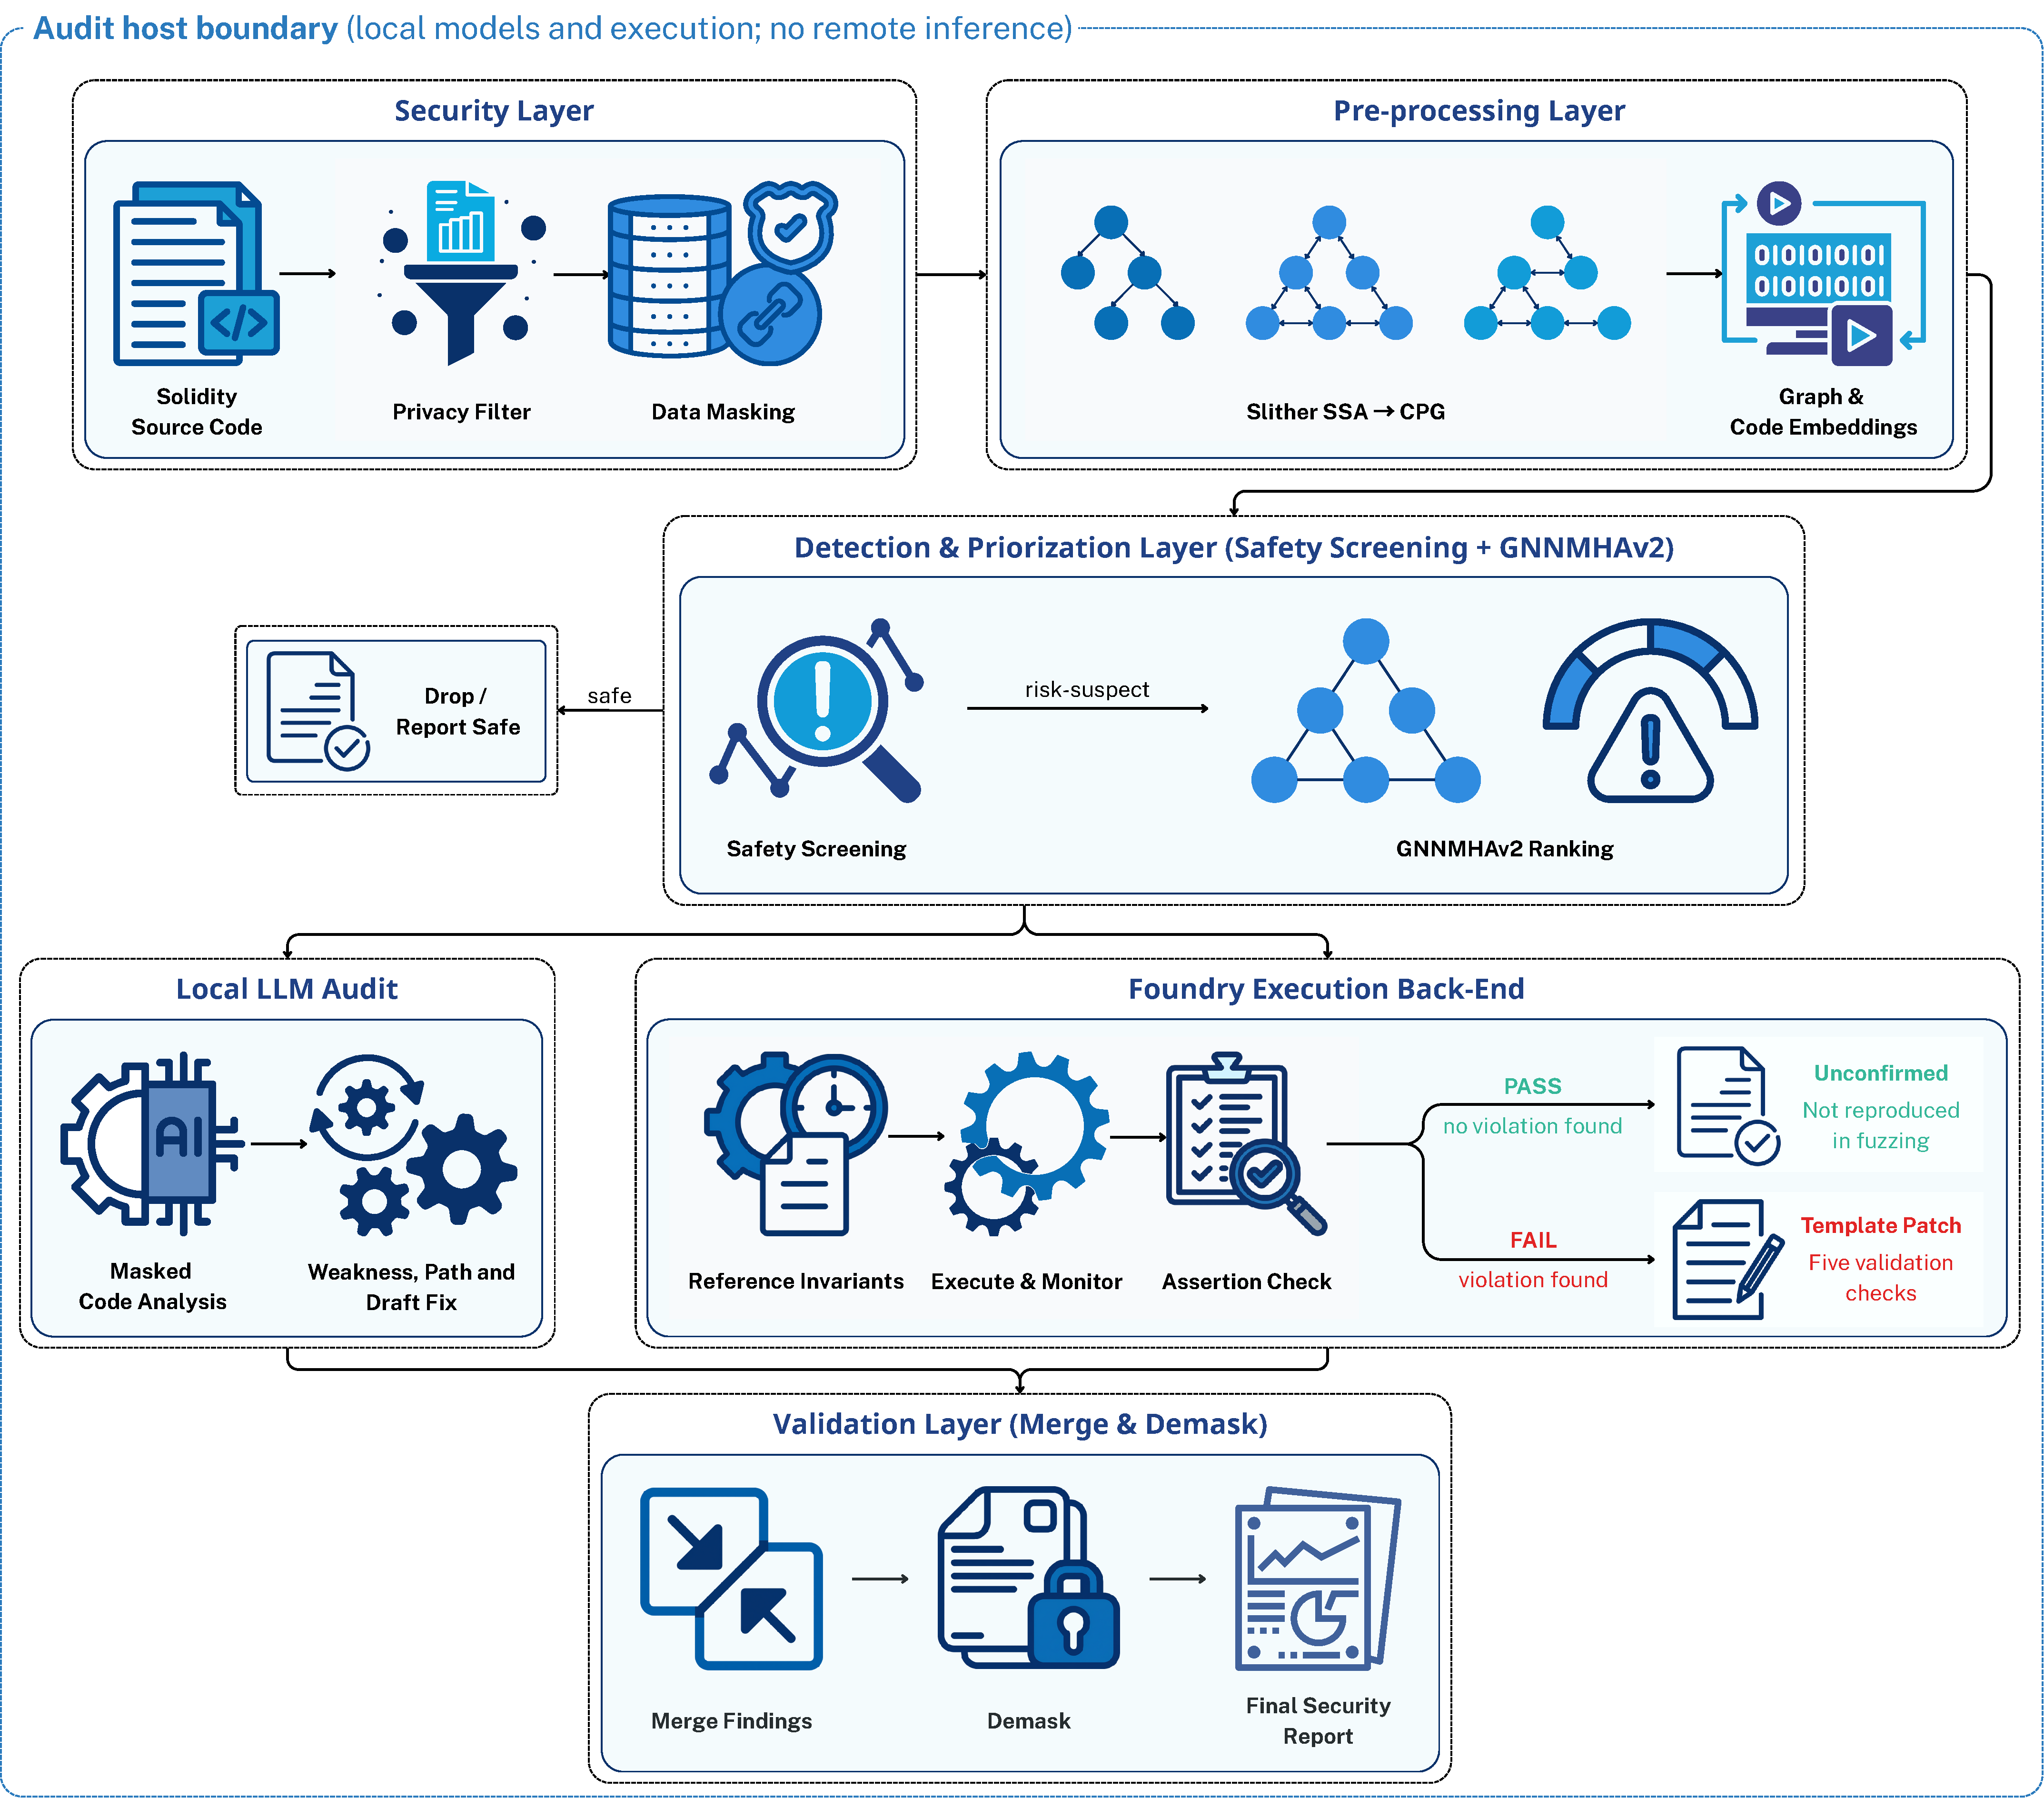
\includegraphics[width=0.84\textwidth]{figures/prism_architecture.pdf}
\caption{PRISM architecture. All eight stages run inside the audit host. Ranked functions are audited by a local open-weight LLM, whose findings are hypotheses, and exercised by Foundry invariant harnesses, which confirm a finding only through a failing assertion. $\mathcal{T}$: pseudonymization map; $\Phi$: ranking score; $\tau$: forwarding threshold.}
\label{fig:pipeline}
\end{figure}

Figure~\ref{fig:pipeline} shows the pipeline; no network access is required once the model weights are installed.

\subsection{Threat Model and Pseudonymization}
\label{sec:threat}

\textit{Assets and trust boundary.} The asset is unreleased contract source code together with the business logic it reveals: identifier names, constants, addresses and endpoints. The trust boundary is the audit host operated by the contract owner or its auditor.

\textit{Adversaries.} We consider (A1) third-party model providers and network observers, to which a cloud-LLM workflow would expose code, and (A2) honest-but-curious parties that later see PRISM artifacts outside the host, such as prompt logs, generated harnesses, bug reports shared with external reviewers, or a shared inference server inside the organization. PRISM removes A1 by construction, since no inference is remote, and DataMasker reduces what A2 learns from artifacts. A fully compromised audit host is out of scope, because such an adversary can read the plaintext source directly.

\textit{Mechanism.} \textit{PrivacyFilter} first removes hard-coded private keys and application programming interface (API) keys, remote procedure call (RPC) endpoints and 20-byte addresses. \textit{DataMasker} then renames user-defined identifiers of contracts, types, functions and variables, and leaves Solidity keywords, EVM built-ins such as \texttt{msg.sender} and \texttt{block.timestamp}, standard interfaces such as \texttt{IERC20}, numeric literals and comments untouched. The $i$-th distinct identifier $x_i$ is mapped to
\begin{equation}
\mathcal{T}(x_i) = \texttt{prism\_}\,\sigma(x_i)\,\texttt{\_}\langle i\rangle,
\end{equation}
where $\langle i\rangle$ is a four-digit counter and $\sigma(x)\in\{\texttt{Type},\texttt{b},\texttt{v}\}$ keeps a coarse lexical role: \texttt{Type} for capitalized names, \texttt{b} for boolean-style names beginning with \emph{is}, \emph{has} or \emph{can}, and \texttt{v} otherwise. $\mathcal{T}$ is a bijection; its inverse $\mathcal{T}^{-1}$ never leaves the host and is applied only to the final report. Sect.~\ref{sec:rq3} measures what $\mathcal{T}$ preserves and what it still reveals to A2.

\subsection{Function-Level Code Property Graph}

From the pseudonymized source $S_{\mathit{mask}}$, PRISM extracts Slither's SSA IR~\cite{feist2019slither} and builds one directed graph per function, $\mathcal{G}=(\mathcal{V},\mathcal{E},X,E_{\mathit{attr}})$, whose nodes are SSA instructions.
\begin{itemize}
\item \textbf{Node features} $X\in\mathbb{R}^{N\times 32}$: a 13-dimensional one-hot instruction type, 10 security indicators (low-level calls, storage reads and writes, guards, transaction-context reads, etc.), and 9 structural attributes (in- and out-degree, loop membership, relative depth, etc.).
\item \textbf{Edge attributes} $E_{\mathit{attr}}\in\{0,1\}^{|\mathcal{E}|\times 4}$: a one-hot edge type among \texttt{sequential}, \texttt{branch}, \texttt{loop\_back} (control flow) and \texttt{data\_dep} (def-use), so that control and data flow share one edge set.
\end{itemize}

\subsection{Two-Stage Graph Attention Ranker}
\label{sec:ranker}

Both stages use the same encoder, GNNMHAv2, which projects node features to $d=256$ dimensions and stacks $L=4$ edge-aware graph attention layers with $K=8$ heads~\cite{velivckovic2017graph,brody2021attentive}. With edge attribute $\mathbf{e}_{ij}$ and $\mathcal{N}^{+}(i)=\mathcal{N}(i)\cup\{i\}$, head $k$ of layer $l$ computes
\begin{equation}
\alpha_{ij}^{k,l}=\operatorname*{softmax}_{j\in\mathcal{N}^{+}(i)}\Big(\mathbf{a}^{k,l\top}\mathrm{LeakyReLU}\big(W_{s}^{k,l}h_i^{l}+W_{t}^{k,l}h_j^{l}+W_{e}^{k,l}\mathbf{e}_{ij}\big)\Big),
\end{equation}
\begin{equation}
h_i^{l+1}=\mathrm{ELU}\Big(\mathrm{BN}\Big(\tfrac{1}{K}\textstyle\sum_{k=1}^{K}\sum_{j\in\mathcal{N}^{+}(i)}\alpha_{ij}^{k,l}\,W^{k,l}h_j^{l}\Big)\Big)+h_i^{l},
\end{equation}
where BN is batch normalization and ELU the exponential linear unit. Residual connections and a jumping-knowledge (JK) readout, $z_i=[h_i^{1}\|h_i^{2}\|h_i^{3}\|h_i^{4}]\in\mathbb{R}^{1024}$, keep both local and multi-hop patterns. The graph embedding $g\in\mathbb{R}^{2048}$ concatenates attention pooling and mean pooling,
\begin{equation}
g=\Big[\textstyle\sum_{i}\beta_i z_i \,\Big\|\, \frac{1}{N}\sum_i z_i\Big],\qquad \beta_i=\operatorname*{softmax}_i\big(\mathbf{w}^{\top}\mathrm{ReLU}(W_p z_i)\big),
\end{equation}
and a two-hidden-layer perceptron maps $g$ to class logits. One layer costs $O(K(|\mathcal{V}|d^2+|\mathcal{E}|d))$, which is linear in graph size for fixed $d$.

Stage~A is a binary model (vulnerable or safe) trained with class-weighted, label-smoothed cross-entropy (CE). Stage~B is a five-class model trained with class-weighted focal loss on label-smoothed CE, with smoothing $\epsilon=0.05$ and $\gamma=2$:
\begin{equation}
\mathcal{L}=\frac{1}{n}\sum_{m=1}^{n}\alpha_{y_m}(1-p_{m})^{\gamma}\,\mathrm{CE}_{\epsilon}(g_m,y_m),
\end{equation}
where $p_m$ is the predicted probability of the true class and $\alpha_{y}$ the class weight. At inference, Stage~A drops functions it predicts safe, Stage~B assigns a class to the remaining ones, and PRISM ranks them by the Stage-B confidence $\Phi(\mathcal{G})=\max_c p_B(c\mid\mathcal{G})$, forwarding functions with $\Phi\ge\tau$ ($\tau=0.3$) in decreasing order of $\Phi$.

\subsection{Local LLM Audit, EVM Execution and Repair}
\label{sec:llm}

\textit{Local LLM audit.} The masked source and the ranked functions, each with its predicted class and $\Phi$, are passed to an open-weight code LLM, DeepSeek-Coder-V2-Lite-Instruct, a 16B-parameter mixture-of-experts model with 2.4B active parameters~\cite{zhu2024deepseek}. It is served on the host by Ollama\footnote{\url{https://ollama.com}; the quantized model occupies 8.3\,GiB on disk.} with temperature 0.1 and at most 4,096 generated tokens. The prompt asks for a structured finding per suspected weakness: weakness type, severity, affected function, attack path, exploit scenario and fix. PRISM treats these findings as hypotheses.

\textit{Execution.} To verify findings dynamically without network calls, PRISM interfaces with a local Foundry execution back end. For evaluated classes, invariant harnesses are instantiated from class templates (e.g., balance conservation for reentrancy, privileged rejection for access control) and fuzzed locally. We benchmark execution using canonical reference harnesses (Sect.~\ref{sec:rq2}) and an empirical safe-case replay (Sect.~\ref{sec:rq4}); automated harness synthesis across arbitrary contracts remains an open challenge (Sect.~\ref{sec:discussion}). A finding is confirmed only if an assertion fails with a concrete counterexample trace.

\textit{Repair and report.} A template-based repair module proposes a patch for each finding, which must pass five checks (Sect.~\ref{sec:rq5}). LLM hypotheses and execution results are merged and deduplicated by function and weakness type, and identifiers are restored through $\mathcal{T}^{-1}$ only in the final report.

%======================================================================
\section{Experimental Setup}
\label{sec:setup}

\subsubsection{\hspace*{\parindent}Research questions (RQs).}
\textbf{RQ1}: How accurately does the ranker classify vulnerable functions, on seen and unseen contract lineages, and how does it compare with other graph learners?
\textbf{RQ2}: Does the local EVM back end execute harnesses reliably and reproducibly?
\textbf{RQ3}: Does pseudonymization preserve analysis utility, and what does it still reveal?
\textbf{RQ4}: How far do taxonomy- and severity-aware filters reduce alarms on safe contracts without losing vulnerable ones?
\textbf{RQ5}: Do template patches block exploits while preserving interfaces?

\subsubsection{\hspace*{\parindent}Dataset.}
We extract 12,991 function-level CPGs with at least three nodes from three public sources: SmartBugs Wild~\cite{durieux2020empirical} (1,179 graphs), the SolidiFI benchmark~\cite{ghaleb2020effective} (8,105 graphs) and LISA-Bench\footnote{AgentLISA: LISA-Bench: Smart contract vulnerability detection benchmark. \url{https://github.com/agentlisa/bench} (2025), accessed September 2026.} (3,707 graphs), a collection of professional audit findings. The graphs cover five classes of the Smart Contract Weakness Classification (SWC) registry: Reentrancy (SWC-107, 2,475), Integer Overflow (SWC-101, 2,392), Access Control (SWC-105, 2,026), Unchecked Return Value (SWC-104, 2,983) and Timestamp / Transaction-Order Dependence (SWC-114, 3,115). Graphs of the remaining source categories (denial of service, delegatecall) are excluded from the five-class task.
Labels follow a contract-derived weak-supervision policy: SmartBugs and SolidiFI functions inherit the label of their contract, and LISA-Bench functions inherit the label obtained by keyword mapping of the finding text. We audited this choice on SolidiFI: of 9,369 injected bug spans in its 350 BugLog contracts, 4,947 map uniquely to a function body, and a strictly span-mapped subset would keep only 2,580 graphs with two Reentrancy and two timestamp dependence examples, too few for a five-class task. The resulting label noise is discussed in Sect.~\ref{sec:discussion}. Stage~A uses all 24,454 graphs as a binary task (labels 0--7 vulnerable; 8 safe).

\subsubsection{\hspace*{\parindent}Splits.}
We use two frozen protocols for the five-class ranker: (i)~\emph{Random split}: stratified 70/15/15 (9,093/1,949/1,949 graphs); and (ii)~\emph{lineage-disjoint split}: contracts are partitioned by origin so that SolidiFI \texttt{buggy\_N} variants, functions from the same LISA-Bench finding, and functions from the same imported source contract never cross partitions, giving 8,349/2,496/2,146 graphs with zero lineage overlap. Stage~A instead uses a frozen binary 70/15/15 split (17,118/3,667/3,669; test: 3,132 vulnerable, 537 safe).

\subsubsection{\hspace*{\parindent}Baselines.}
To isolate the effect of the encoder, we train graph convolutional (GCN) and graph isomorphism (GIN) networks as well as GAT and GATv2 on the same graphs, node features, splits and training budget; GAT and GATv2 do not use edge attributes. As a rule-based reference, Slither~0.11.5 is mapped to the five classes through its detector names (e.g., \texttt{reentrancy-eth} to Reentrancy, \texttt{unchecked-lowlevel} to Unchecked Return), and a function that triggers no mapped detector is assigned the majority training class.

\subsubsection{\hspace*{\parindent}Implementation.}
Models are implemented in PyTorch Geometric and trained with AdamW (learning rate $10^{-3}$, weight decay $10^{-4}$), batch size 64 and OneCycleLR for up to 35 epochs with early stopping on validation macro-F1 (patience 15). GNNMHAv2, GCN and GIN are trained with five seeds (42 to 46); GAT and GATv2 with seed 42. Experiments run on an Apple M4 CPU (10 cores, 16\,GB RAM). One 35-epoch training run of GNNMHAv2 takes $348.3\pm37.2$\,s, compared with $56.5\pm6.7$\,s for GCN and $67.4\pm1.3$\,s for GIN, and inference takes 0.21\,ms per function graph. Execution uses Foundry Forge~1.5.1 and \texttt{solc}~0.8.30.

%======================================================================
\section{Results}
\label{sec:results}

\subsection{RQ1: Function-Level Ranking Accuracy}
\label{sec:rq1}

\begin{table}[t]
\centering
\caption{Comparison with graph baselines on both splits (five-seed mean $\pm$ std). Single-seed GAT and GATv2 score within 0.5 points of GNNMHAv2 (0.7562 and 0.7571). Slither is mapped to the five classes. Best mean per column in bold.}
\label{tab:baselines}
\resizebox{\linewidth}{!}{%
\begin{tabular}{lcccc}
\toprule
& \multicolumn{2}{c}{Random split ($n=1{,}949$)} & \multicolumn{2}{c}{Lineage-disjoint split ($n=2{,}146$)} \\
\cmidrule(lr){2-3}\cmidrule(lr){4-5}
Method & Accuracy & Macro-F1 & Accuracy & Macro-F1 \\
\midrule
Slither 0.11.5 (mapped)           & 0.2299 & 0.0748 & 0.2330 & 0.0756 \\
GCN (5 seeds)                     & 0.7434 $\pm$ 0.0016 & 0.7604 $\pm$ 0.0022 & \textbf{0.7445} $\pm$ 0.0008 & 0.7630 $\pm$ 0.0009 \\
GIN (5 seeds)                     & \textbf{0.7442} $\pm$ 0.0005 & \textbf{0.7609} $\pm$ 0.0005 & 0.7432 $\pm$ 0.0011 & 0.7617 $\pm$ 0.0011 \\
GNNMHAv2 (PRISM, 5 seeds)         & 0.7426 $\pm$ 0.0014 & 0.7595 $\pm$ 0.0019 & \textbf{0.7445} $\pm$ 0.0006 & \textbf{0.7631} $\pm$ 0.0006 \\
\bottomrule
\end{tabular}%
}
\end{table}

Table~\ref{tab:baselines} compares the ranker with graph baselines. GNNMHAv2 reaches $0.7595\pm0.0019$ macro-F1 on the random split and $0.7631\pm0.0006$ on the lineage-disjoint split, with macro-precision $0.887\pm0.005$ and macro-recall $0.725\pm0.001$ on the random split. The mapped Slither reference scores $0.0748$ because its detectors fire on few function slices under our label mapping. Over five fresh seeds, Stage~A reaches $88.62\pm0.24\%$ accuracy ($87.82\pm0.32\%$ vulnerable recall; $93.26\pm0.61\%$ safe specificity; $n=3{,}669$).

The more informative result is that all graph learners converge to the same level. On both splits, GCN, GIN, GAT, GATv2 and GNNMHAv2 lie within 0.5 macro-F1 points of each other. In 20 paired exact McNemar tests between GNNMHAv2 and GCN or GIN (two splits, five seeds), no difference is significant (all $p>0.16$), the paired models disagree on at most 22 test functions per run, and between 97.4\% and 99.6\% of GNNMHAv2's errors are shared with the baseline. Pairwise Jaccard error overlap exceeds 96.5\%, and 493 of 520 errors (94.8\%) are shared across all five architectures. When diverse models make identical errors, the result is consistent with label noise being a stronger limitation than encoder choice. A structural-label-conflict diagnostic confirms this: 6.2\% of random-split test graphs match a training graph with a conflicting label due to contract-level inheritance; on these conflicting graphs, accuracy collapses to 7.9\%, whereas on conflict-free graphs it reaches 78.7\%.

\begin{figure}[t]
\centering
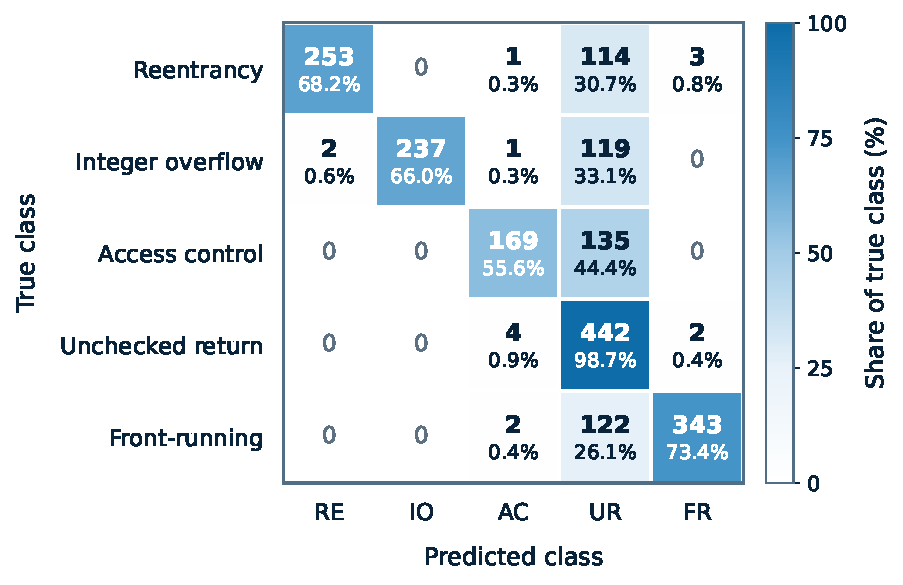
\includegraphics[width=78mm]{figures/confusion_matrix_5class_en.pdf}
\caption{Confusion matrix of a single GNNMHAv2 training run on the frozen random split (seed 42; $n=1{,}949$; accuracy 0.7414, macro-F1 0.7581; five-seed results are in Table~\ref{tab:baselines}). Cells show counts and the share of the true class. Columns follow the row order: Reentrancy (RE, SWC-107), Integer overflow (IO, SWC-101), Access control (AC, SWC-105), Unchecked return (UR, SWC-104), Timestamp dependence (TD, SWC-114).}
\label{fig:confusion}
\end{figure}

The per-class view in Fig.~\ref{fig:confusion} shows where the shared errors go. Precision is 0.95 to 1.00 for the four specific classes, but their recall is 0.56 to 0.73, and 490 of the 505 errors are predictions of \emph{unchecked return} (precision 0.47, recall 0.99), whose SSA signature, an external call followed by an unused result, is the most generic. The model therefore rarely confuses two specific weaknesses. It assigns functions that carry no class-specific evidence to the most generic class, which is what contract-derived labels produce when a contract's label is inherited by functions that do not contain the flaw. Consistently, top-2 accuracy (five-seed mean) is 0.8086, so the second-ranked class recovers only 25.6\% of the errors: most errors are not near misses.

\begin{table}[t]
\centering
\small
\caption{Ablation of GNNMHAv2 on the random split (five seeds, mean $\pm$ std). $\Delta$: change in mean macro-F1 relative to the full model.}
\label{tab:ablation}
\begin{tabular}{lccc}
\toprule
Variant & Macro-F1 & $\Delta$ & Top-2 accuracy \\
\midrule
Full model                       & 0.7595 $\pm$ 0.0019 & -- & 0.8086 \\
without edge attributes          & 0.7603 $\pm$ 0.0011 & +0.0008 & 0.8085 \\
without jumping knowledge        & 0.7597 $\pm$ 0.0018 & +0.0002 & 0.8117 \\
focal loss $\rightarrow$ cross-entropy & 0.7584 $\pm$ 0.0012 & $-$0.0010 & 0.8097 \\
attention+mean $\rightarrow$ mean pooling & 0.7596 $\pm$ 0.0029 & +0.0001 & 0.8115 \\
$L=2$                            & 0.7611 $\pm$ 0.0016 & +0.0016 & 0.8079 \\
$L=3$                            & 0.7588 $\pm$ 0.0025 & $-$0.0007 & 0.8069 \\
$K=4$                            & 0.7588 $\pm$ 0.0017 & $-$0.0007 & 0.8089 \\
\bottomrule
\end{tabular}
\end{table}

The ablation in Table~\ref{tab:ablation} supports the same reading. Removing edge attributes, jumping knowledge or attention pooling, replacing focal loss, and changing depth or head count all move macro-F1 by at most 0.16 points, within one to two standard deviations of seed variation. Under contract-derived labels, encoder design is not the bottleneck; label granularity is. For PRISM this has a practical consequence. The ranker's job is to order functions for later stages, any of these encoders does so at the same quality, and at 0.21\,ms per function the choice costs nothing next to execution. Better labels, not a larger encoder, are the lever for better ranking.

\subsection{RQ2: Execution Back-End Reliability}
\label{sec:rq2}

We executed expert-written reference harnesses for five case-study contracts under 30 fuzzing seeds (101 to 130) in a directed exploit test and a 10,000-call fuzzing campaign, for $5\times30\times2=300$ runs. The targets cover the taxonomy: SimpleDAO (SWC-107, reentrancy), TokenSale (SWC-101, integer overflow), UnprotectedVault (SWC-105, access control), UncheckedBank (SWC-104, unchecked return), and TimestampLock (SWC-114, timestamp dependence). All 300/300 runs passed without timeouts (mean directed/fuzz latency 190.26/202.75\,ms); directed transaction gas was deterministic at 77,558, 39,648, 48,550, 27,202 and 39,827, respectively. A seed-42 integrated trace ran masking, preprocessing, GNN routing, bounded local LLM audit and reference tests for all five cases; every stage completed and 5/5 directed and 10,000-call tests passed. It demonstrates orchestration, not automated harness generation or benchmark-wide end-to-end performance. Because the harnesses are hand-written, RQ2 does not measure generated-harness bug-finding frequency (Sect.~\ref{sec:discussion}).

\subsection{RQ3: Pseudonymization Fidelity and Residual Exposure}
\label{sec:rq3}

\begin{table}[t]
\centering
\small
\caption{DataMasker on the 57 benchmark contracts (286 user-defined identifiers). Upper block: utility (higher is better). Lower block: exposure to an A2 adversary (lower is better).}
\label{tab:datamasker_eval}
\begin{tabular}{lrl}
\toprule
Metric & Value & Meaning \\
\midrule
Compilation validity             & 57/57 (100\%)   & masked code compiles \\
Exact restoration                & 57/57 (100\%)   & $\mathcal{T}^{-1}$ restores the source \\
Slither detector types retained  & 229/229 (100\%) & per contract; 6 added \\
\midrule
Dictionary exposure              & 87/286 (30.4\%)  & name in a 32-term domain list \\
Frequency re-linkage             & 256/286 (89.5\%) & rank matching of counts \\
\bottomrule
\end{tabular}
\end{table}

\textit{Utility.} Table~\ref{tab:datamasker_eval} shows that DataMasker is lossless for compilation and restoration: every masked contract compiles with \texttt{solc}, and $\mathcal{T}^{-1}$ restores every contract exactly. For static analysis, all 229 contract-level Slither detector types raised on plaintext code are preserved on masked code (235 total; six added by naming conventions). Under taxonomy-guided auditing across the five SWC classes, raw-code recall on the 30 vulnerable contracts reaches 30/30 (100.0\%) with 11/27 (40.7\%) safe specificity, showing that unconstrained LLM inspection raises substantial false alarms on benign patterns. On pseudonymized code, masked recall achieves 13/30 (43.3\%) while safe specificity increases to 19/27 (70.4\%). This unguided text-only baseline drops recall when role-revealing names (e.g., \texttt{owner}) are masked, demonstrating why PRISM couples local LLMs with structural GNN screening to isolate suspicious slices without relying on identifier semantics. Crucially, across all contracts with EVM built-ins (\texttt{block.timestamp}, external \texttt{.call}), raw and masked hypotheses achieve identical predictions ($J=1.00$).

\textit{Exposure.} We quantify two A2 adversaries. The \emph{dictionary} measure counts identifiers whose plaintext name is one of 32 common Solidity and DeFi terms (e.g., \texttt{owner}, \texttt{balance}, \texttt{withdraw}); an adversary who guesses these terms from the role of a pseudonym recovers at most 30.4\% of identifiers. The \emph{frequency} adversary knows how often each plaintext identifier occurs in the contract, for example from an earlier version or a leaked excerpt, ranks identifiers and pseudonyms by occurrence count, and aligns the two rankings. Because $\mathcal{T}$ renames one-to-one and preserves occurrence counts, only ties stop it, and it re-links 89.5\% of identifiers. This is an upper bound under strong side knowledge, and it is the informative result: renaming preserves the structure of the code, so pseudonymization alone is not a confidentiality mechanism for code sent to an untrusted model, in line with learned name recovery from binaries~\cite{xie2024resym,xu2025gennm}. It is defense in depth for artifacts that leave the host, and this measurement is why PRISM keeps inference local instead of masking code and sending it to a hosted LLM.

\subsection{RQ4: Alarm Reduction on Safe Contracts}
\label{sec:rq4}

We ran Slither~0.11.5 on the 57-contract benchmark (27 safe and 30 vulnerable contracts, labeled by their benchmark templates) and applied PRISM's static filters in sequence (Table~\ref{tab:cascade_routing}).

\begin{table}[t]
\centering
\caption{Alarms along the \emph{static} filtering cascade on 57 contracts. ``Safe cleared'' measures contract-level specificity; ``Vuln.\ retained'' tracks preservation of Slither-flagged vulnerable contracts.}
\label{tab:cascade_routing}
\small
\setlength{\tabcolsep}{2.2pt}
\begin{tabular}{llrrr}
\toprule
Stage & Filter & Alarms & Safe cleared ($\uparrow$) & Vuln.\ retained \\
\midrule
0 & Slither, all detectors                 & 230 & 0/27 (0.0\%)          & 30/30 (100\%) \\
1 & Five target SWC classes only           & 41  & 21/27 (77.8\%)        & 18/30 (60.0\%) \\
2 & High/medium impact, confidence         & 33  & 21/27 (77.8\%)        & 18/30 (60.0\%) \\
\bottomrule
\end{tabular}
\end{table}

Unfiltered Slither raises 230 alarms and flags every contract, yielding 0/27 (0.0\%) specificity and 30/57 (52.6\%) precision due to stylistic detectors. Restricting output to the five target classes (Stage~1) clears 21 of 27 safe contracts (77.8\% specificity); 12 vulnerable contracts lack dedicated Slither detectors under this mapping. Filtering for high/medium impact and confidence (Stage~2) eliminates eight secondary/low-severity alarms on already-flagged contracts, preserving contract-level specificity (21/27) while retaining all 18 detected flaws. Separately, template-based execution validation on 57 labeled benchmark fixtures (20.90\,s in Foundry under \texttt{solc}~0.8.30) ran deterministically: 30 labeled vulnerable fixtures satisfy exploit predicates and 27 safe fixtures satisfy safety predicates, confirming concrete EVM feasibility while automated synthesis for arbitrary mainnet test suites remains future work.

\subsection{RQ5: Patch Validation}
\label{sec:rq5}

For the five case-study contracts with exploit harnesses (Sect.~\ref{sec:rq2}), template repair produced one patch each. Each patch passed five checks: (1)~compilation with \texttt{solc}~0.8.30; (2)~minimal change ($\le 25\%$ of lines via an AST parse); (3)~the original exploit harness now reverts; (4)~the 10,000-call fuzzing campaign still passes; and (5)~function selectors and storage layout are unchanged, preserving the external ABI and proxy storage layout.

%======================================================================
\section{Discussion and Threats to Validity}
\label{sec:discussion}

Graph screening is linear in graph size, costing 0.21\,ms per function after CPG extraction (negligible next to one Foundry run of 0.19--0.20\,s, Sect.~\ref{sec:rq2}); the LLM stage is invoked only for functions with $\Phi\ge\tau$, bounding generations per contract.

\subsubsection{\hspace*{\parindent}Threats to validity.}
\emph{Construct.} Function graphs inherit contract-derived labels, so benign functions are counted as positives, bounding ranking accuracy. The 57 benchmark labels follow injection templates rather than manual spans, and SWC-114 targets are timestamp proxies. \emph{Internal.} The 57 contracts follow standardized invariant and exploit templates; automated harness synthesis for arbitrary multi-file mainnet contracts remains open work. Slither IR extraction may degrade on inline Yul. DataMasker preserves string literals and comments. \emph{External.} Direct cross-dataset evaluation on LISA-Bench without fine-tuning dropped macro-F1 from 0.8985 to 0.5157. Benchmark contracts are small reference implementations under \texttt{solc}~0.8.30.

\subsubsection{\hspace*{\parindent}Data availability.}
Code, configurations, frozen split manifests, result files and reference harnesses are available in an anonymized repository: \url{https://anonymous.4open.science/r/PRISM-PROJECT/}.

%======================================================================
\section{Conclusion}
\label{sec:conclusion}

This paper presented PRISM, a confidential smart contract audit pipeline keeping every model and artifact on the audit host. Its two-stage graph attention ranker orders functions at $76.31\pm0.06\%$ macro-F1 on unseen lineages in 0.21\,ms per function, showing that contract-derived labels dominate error rather than model capacity. Reversible pseudonymization preserves compilation, restoration, and static analysis, while an 89.5\% frequency re-linkage demonstrates that local inference is essential. Together with reproducible EVM execution, static filtering reducing flagged safe contracts from 27/27 to 6/27, and reference-harness validation on scoped case studies, PRISM makes confidential auditing practical for teams that cannot share code. Future work will expand end-to-end evaluation on larger production benchmarks, replace contract-derived supervision with precise function-level ground truth, and extend template repair to automated multi-harness patch synthesis.

\bibliographystyle{splncs04unsrt}
\bibliography{references}

\end{document}
